% Sección obligatoria.
% ¿Qué escribir en esta sección?
% Se hace un análisis de los resultados obtenidos. Esta sección contiene detalles acerca de cómo y por qué se obtuvieron dichos resultados. 
% Los resultados necesitan una descripción detallada de cómo fueron obtenidos (cuántos intentos, cuántas pruebas y cuántos casos exitosos).

El desarrollo de la solución web de capacitación empresarial basada en
microaprendizaje ha demostrado ser factible, cumpliendo con los objetivos
planteados en el diseño inicial. La solución implementa un sistema flexible
que facilita el acceso al aprendizaje y optimiza el tiempo de formación de los
empleados.

Como resultado, se han implementado módulos clave que permiten personalizar el
contenido educativo, garantizar accesibilidad desde múltiples dispositivos y
facilitar la interacción mediante plataformas externas. Uno de los aspectos
distintivos del sistema es la integración con Telegram.

Integrar el sistema de capacitación con esta plataforma de mensajería ha
permitido ir mejorando la interacción y automatización de notificaciones para
los usuarios. A continuación, se presentan las principales pantallas que
demuestran esta funcionalidad.

\begin{figure}[H]
    \centering
    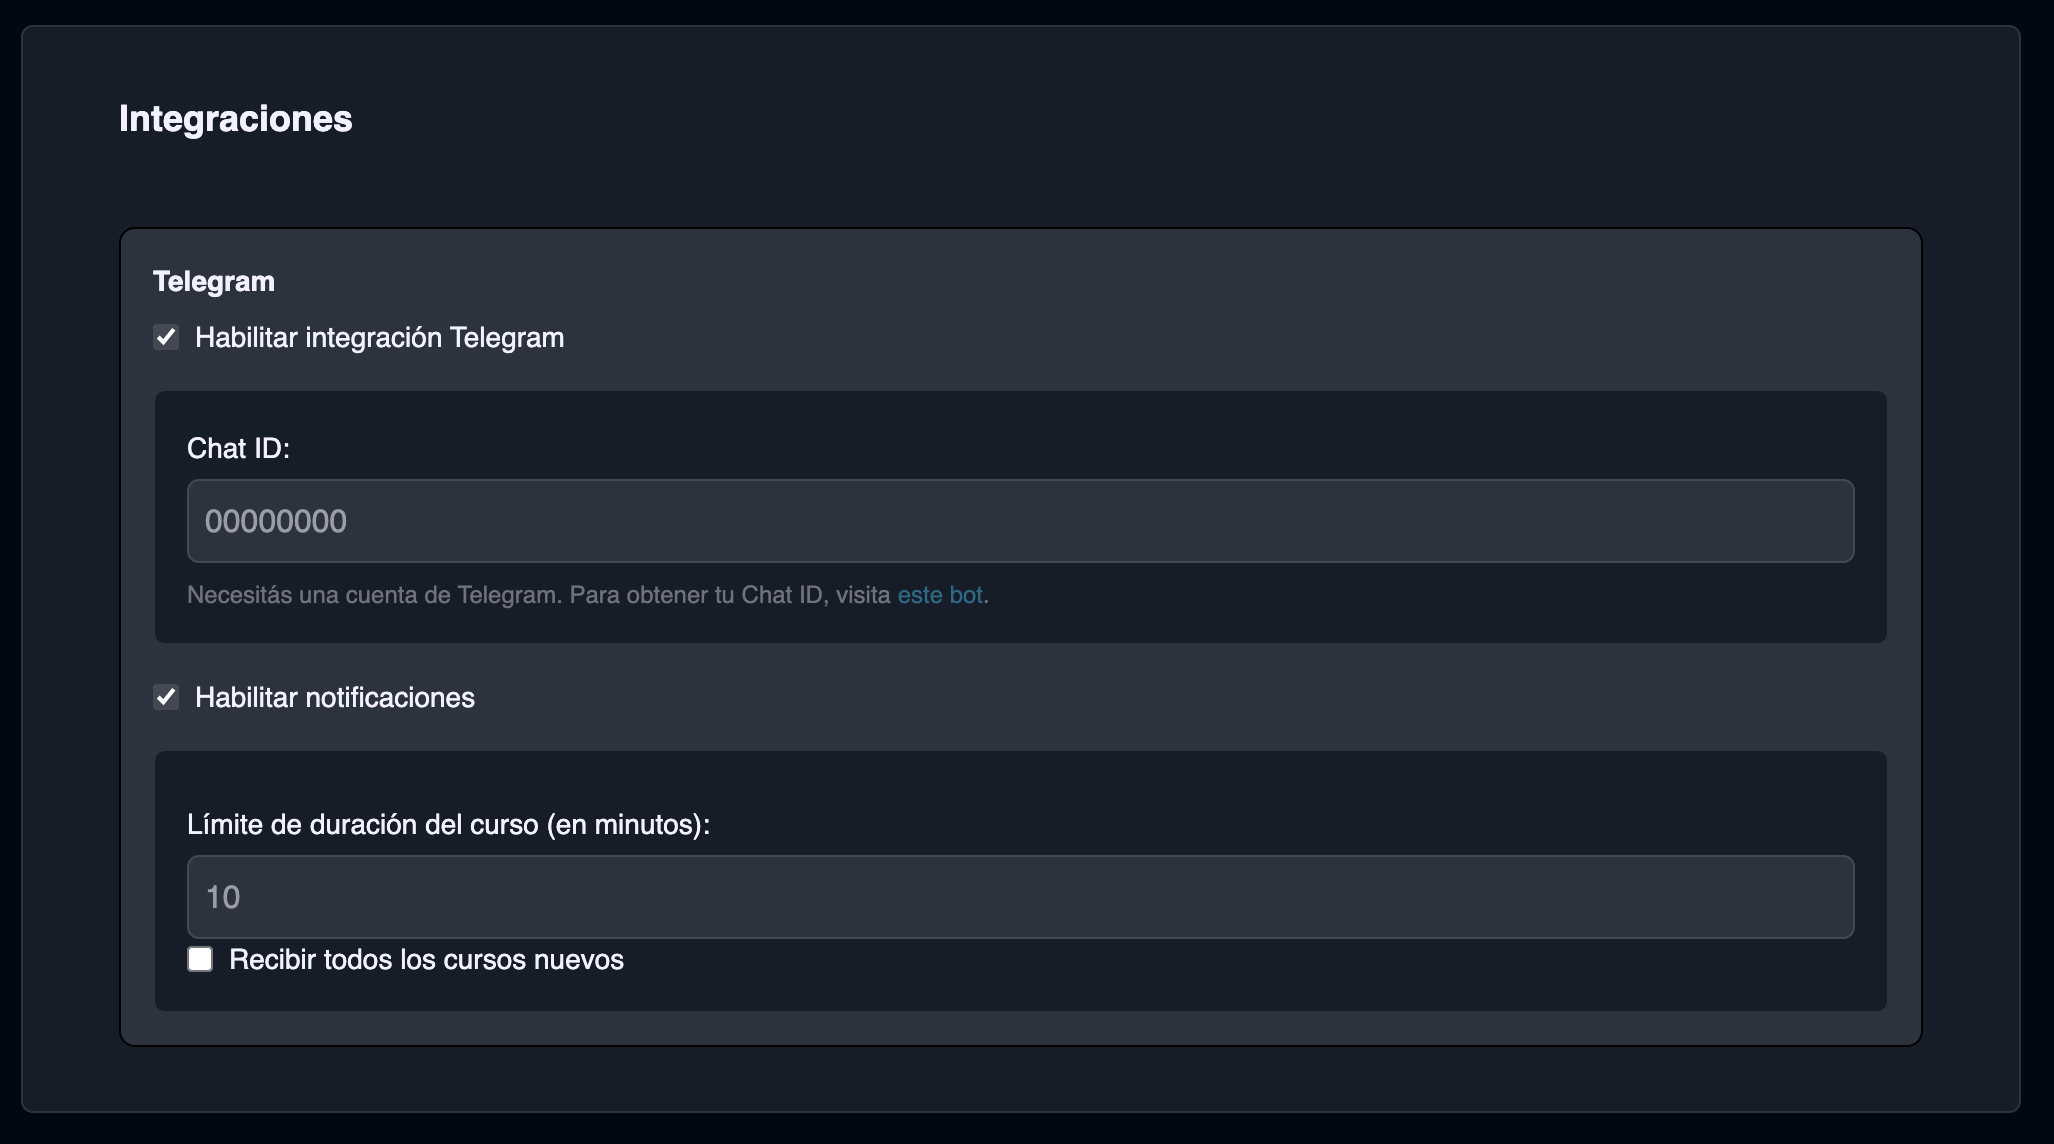
\includegraphics[width=\linewidth]{integracion_telegram/integracion_telegram_02.png}
    \caption{Interfaz del sistema con configuración de integración a Telegram}
    \label{fig:interfaz_integracion_telegram}
\end{figure}

La Figura \ref{fig:interfaz_integracion_telegram} muestra la sección del sistema
donde se encuentra la configuración para integrar Telegram. Desde esta interfaz,
los usuarios pueden activar la funcionalidad y gestionar sus preferencias de
notificación.

\begin{figure}[H]
    \centering
    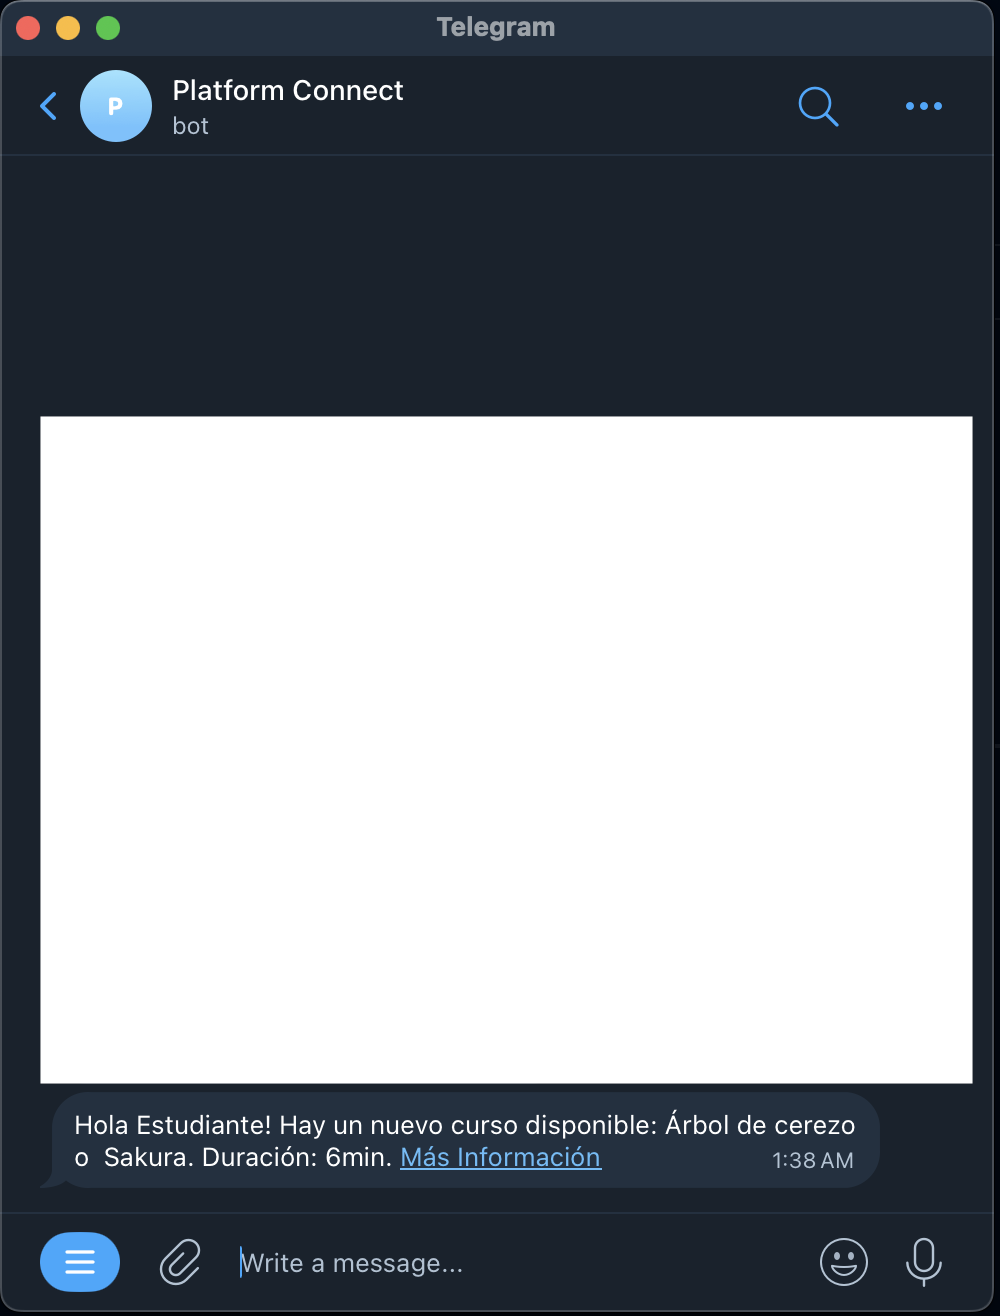
\includegraphics[width=\linewidth]{integracion_telegram/integracion_telegram_05.png}
    \caption{Notificación generada por el sistema en Telegram}
    \label{fig:notificacion_telegram}
\end{figure}

La Figura \ref{fig:notificacion_telegram} presenta una notificación enviada al
usuario a través de Telegram. Estas notificaciones permiten alertar sobre nuevos
cursos disponibles y recordatorios de formación, asegurando una comunicación
eficiente dentro del proceso de aprendizaje.

\begin{figure}[H]
    \centering
    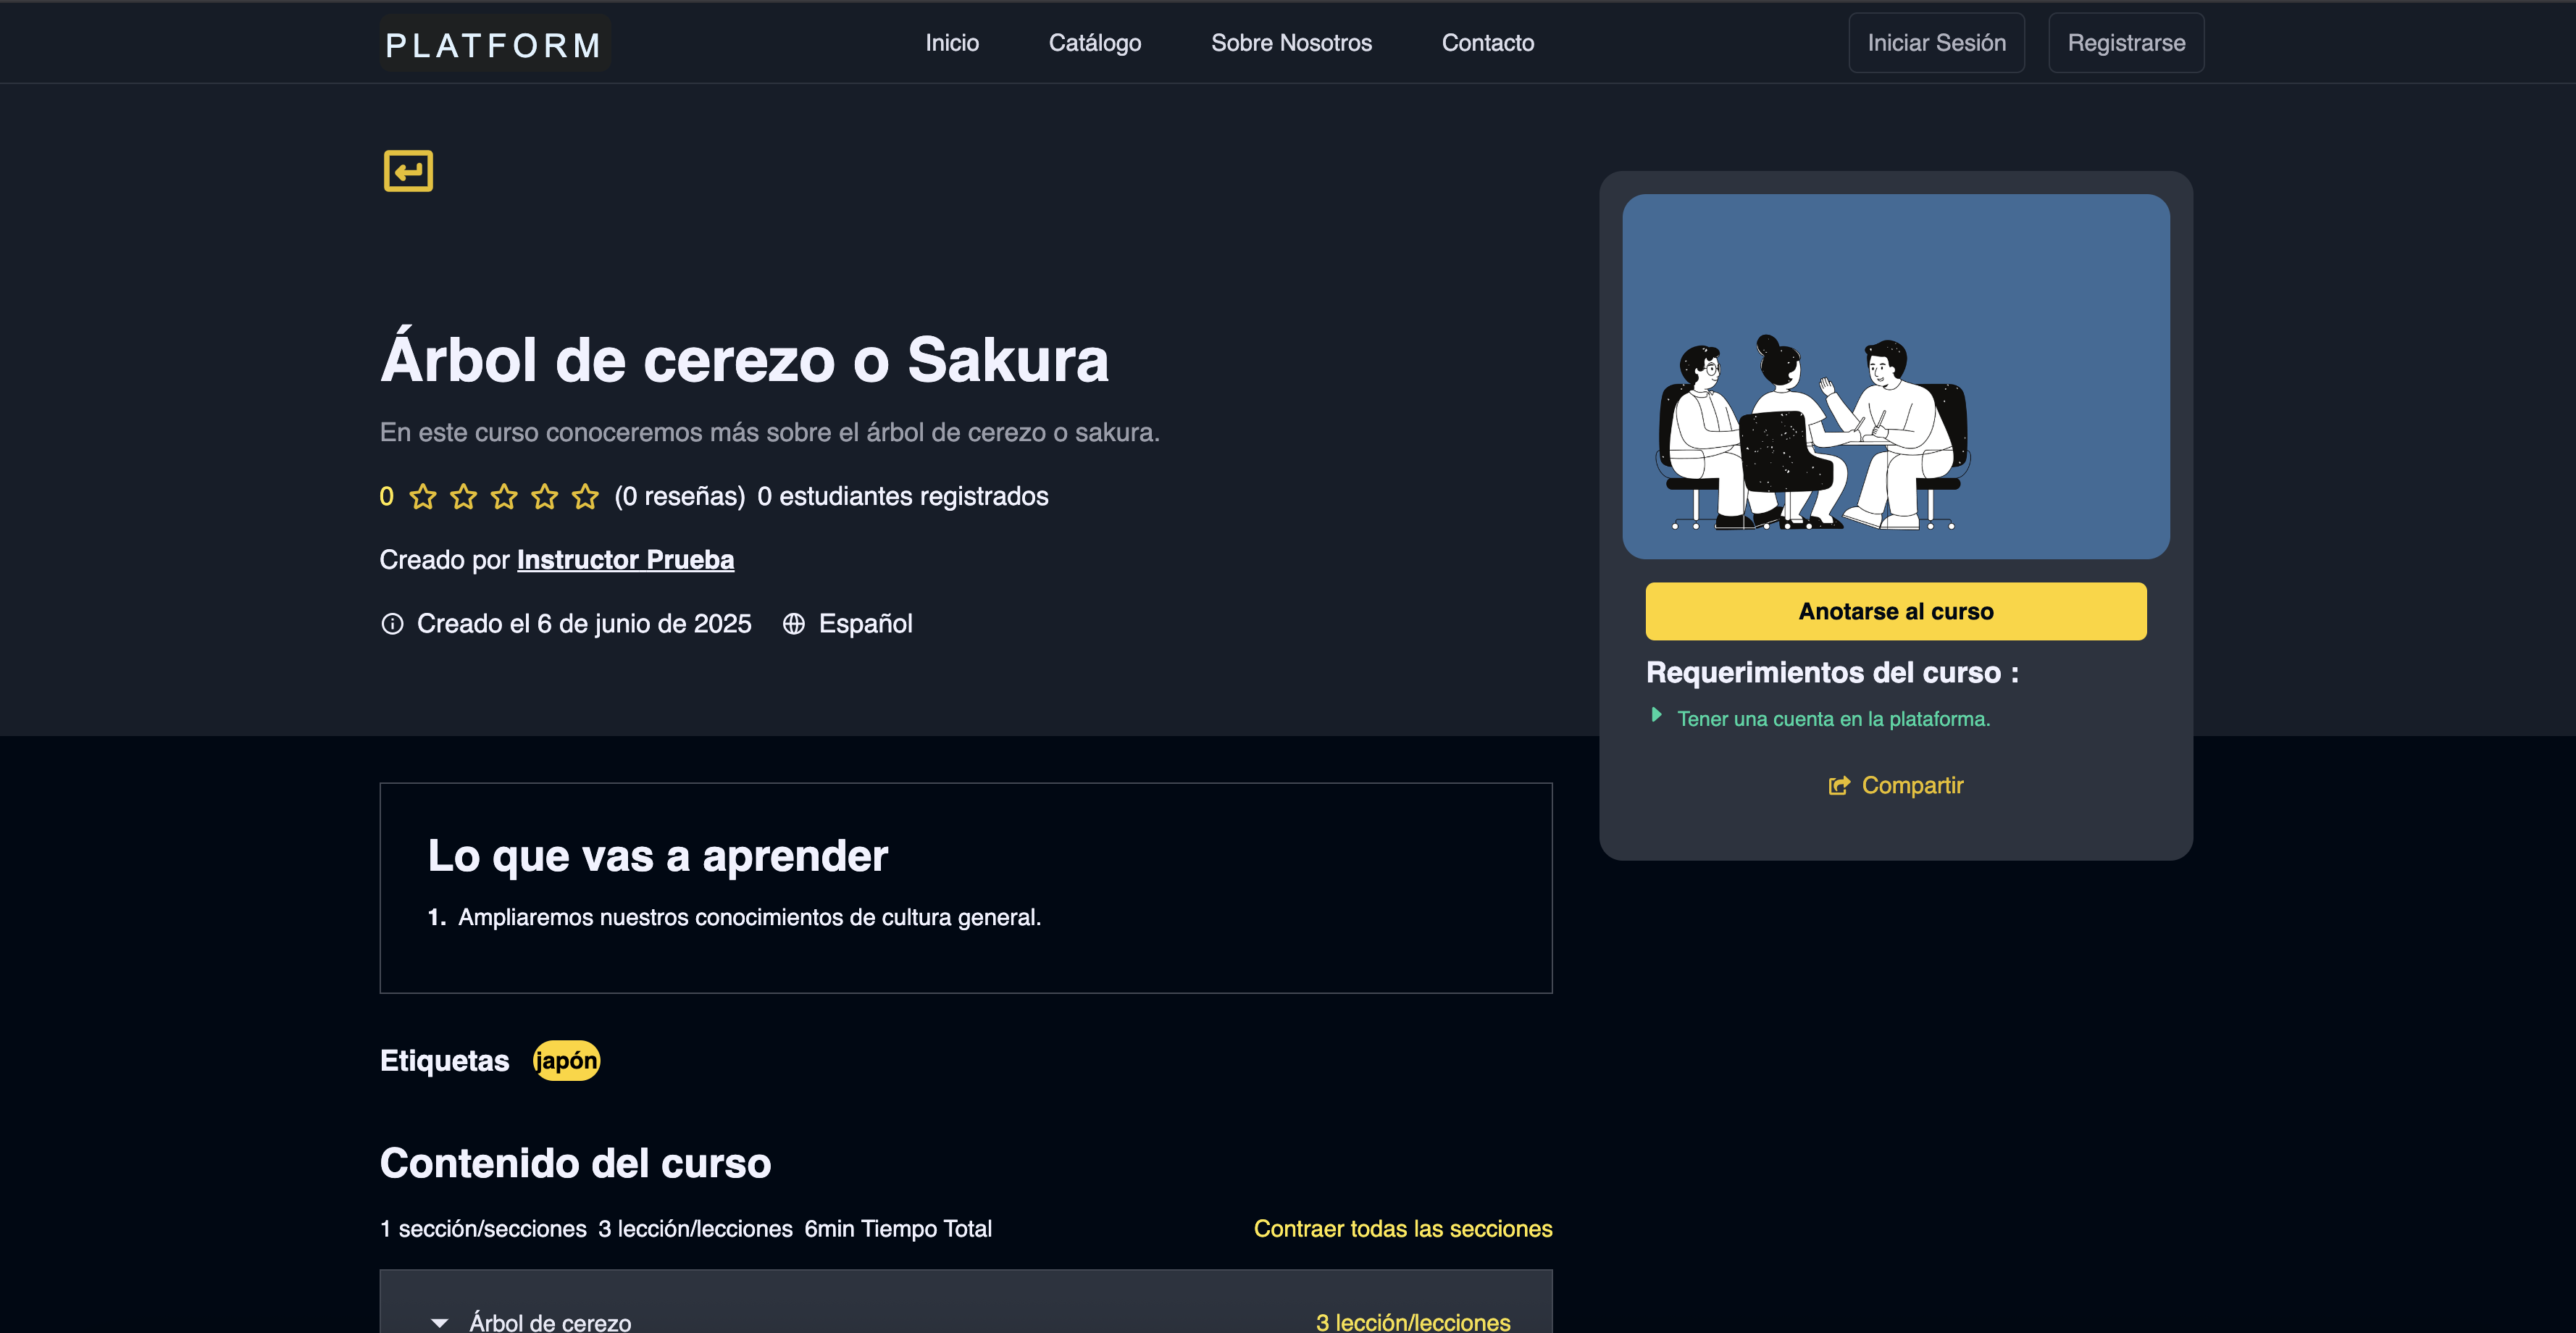
\includegraphics[width=\linewidth]{plataforma/plataforma_07.png}
    \caption{Interfaz del sistema tras acceder desde la notificación}
    \label{fig:interfaz_curso_ejemplo}
\end{figure}

La Figura \ref{fig:interfaz_curso_ejemplo} muestra la vista de un curso al que
el usuario accede tras presionar al enlace provisto por la notificación
recibida en Telegram. Desde esta pantalla, el usuario puede explorar los
detalles del curso y realizar su inscripción de manera rápida, garantizando una
transición fluida entre la plataforma de mensajería y el sistema de
capacitación.

Los principales logros de la solución incluyen:
\begin{itemize}
    \item Personalización del contenido educativo según el perfil y objetivos
    individuales de los empleados.
    \item Integración con plataformas de mensajería para optimizar la
    interacción y accesibilidad.
    \item Accesibilidad multiplataforma, permitiendo el uso desde dispositivos
    móviles y de escritorio.
\end{itemize}

Esto demuestra por un lado la viabilidad del sistema y su capacidad de
adaptación a diversos entornos de capacitación empresarial. Por otro lado, estos
resultados reflejan la integración efectiva del sistema con plataformas
externas, mejorando la accesibilidad y potenciando la experiencia del usuario en
el proceso de aprendizaje.
